\chapter{Persistence Modules}

\section{Persistence modules on $\rr$.}
\begin{definition}
    Let $\cc$ be a category, and denote $(\rr, \le)$
    to be the poset category on $\rr$ with respect to the natural relation 
    $\le$. We define a functor $F: (\rr, \le) \to \cc$ 
    to be a \textbf{persistence module}. 
\end{definition}

Thus we can say that a persistence module is an element of the functor 
category $\cc^{\rr}$. 

A persistence module allows us to model the evolution of objects within some 
category $\cc$. For example, if we have some ascending chain of vector spaces 
\begin{center}
    \begin{tikzcd}[row sep = 1.4cm, column sep = 1.4cm]
        \cdots \arrow[r] & V_{i - 1} \arrow[r] & 
        V_i
        \arrow[r] 
        &
        V_{i+1}
        \arrow[r]
        &
        \cdots
    \end{tikzcd}
\end{center}
then we say that such a chain is a persistence module since it can 
be modeled as a functor from $\rr \to \textbf{Vec}$.  

Let $S = \{s_1, s_2, \dots, s_n\}$ be a finite subset of $\rr^n$. Then we can describe  
an adjunction  
\begin{center}
    \begin{tikzcd}
        \cc^{\rr} \arrow[r, shift left = 0.5ex]
        \arrow[<-, r, shift right = 0.5ex]
        &
        \cc^{S}
    \end{tikzcd}
\end{center}
as follows. First observe that since $S \subset \rr$, there exists
a restriction functor 
$R: \cc^{\rr} \to \cc^{S}$, which acts as a restriction (hence the naming $R$): 
\[
    R(F: \rr \to \cc) = F\big|_{S}: S \to \cc.
\]  
How can we write a functor going in the opposite direction? That is, given a
persistence module which acts on $S$, 

\begin{center}
    \begin{tikzpicture}
        \draw[Red!70, -stealth, <->] (-3, 0) -- (3, 0);
        \node at (3.5, 0) {$\cdots$};
        \node at (-3.5, 0) {$\cdots$};
        \filldraw[Red] (0,0) circle (0.05cm);
        \filldraw[Red] (-0.7,0) circle (0.05cm);
        \filldraw[Red] (-2,0) circle (0.05cm);
        \filldraw[Red] (-0.2,0) circle (0.05cm);
        \filldraw[Red] (1,0) circle (0.05cm);
        \filldraw[Red] (0.8,0) circle (0.05cm);
        \filldraw[Red] (-0.4,0) circle (0.05cm);
        \filldraw[Red] (0.35,0) circle (0.05cm);
        \filldraw[Red] (0.9,0) circle (0.05cm);
        \filldraw[Red] (1.5,0) circle (0.05cm);
        \filldraw[Red] (1.8,0) circle (0.05cm);
        \filldraw[Red] (-1,0) circle (0.05cm);
        \filldraw[Red] (-1.2,0) circle (0.05cm);
        \draw[-stealth, ->] (1.5, 0.5) to [bend left] (3, 1);
        \draw node at (3.3, 1) {$\cc$};
        \draw node at (2.2, 1.3) {$K$};
    \end{tikzpicture}
\end{center}
is there a canonical way to extend this 
to a persistence module which acts on the rest of $\rr$? 
\begin{center}
    \begin{tikzpicture}
        \node at (-3.5, 0) {$\cdots$};
        \draw[NavyBlue, -stealth, <->] (-3, 0) -- (3, 0);
        \node at (3.5, 0) {$\cdots$};
        \draw[-stealth, ->] (3, 0.5)  to [bend left] (5, 1);
        \draw node at (5.3, 1) {$\cc$};
        \draw node at (3.9, 1.4) {$\overline{K}$};
    \end{tikzpicture}
\end{center}

One way we may extend a persistence module $K: S \to \cc$ in $\cc^S$ to 
a persistence module in $\cc^{\rr}$ is to define a functor $\overline{K}: \rr \to \cc$ 
where 
\[
    \overline{K}(r) = 
    \begin{cases}
        I & \text{if } s < s_1\\
        K(r) & \text{if } s_{i} \le r \le s_{i+1}\\
        K(r_n) & \text{if } r > s_n
    \end{cases}
    = 
    \begin{cases}
        I & \text{if } r < \text{min}(S)\\
        K(s_r) & \text{where } s_r \text{ is the largest } s_r \in \text{ S such that } s_r \le r.
    \end{cases}
\]
Now consider a morphism 
$\eta: K \to P$ in $\cc^{S}$; that is, a natural transformation. 
By our above procedure we have a way of discussing the objects $\overline{K}$ 
and $\overline{P}$; but can we obtain a natural transformation 
$\overline{\eta}: \overline{K} \to \overline{P}$ from $\eta$? That is, may we 
extend this relationship to a functor? 

First, observe that we may write $\eta: K \to P$ as follows. 
\begin{center}
    \begin{tikzcd}[row sep = 1.4cm, column sep = 1.4cm]
        P(s_1) 
        \arrow[r] 
        & P(s_2) 
        \arrow[r]
        &
        \cdots
        \arrow[r]
        & P(s_{n-1}) 
        \arrow[r]
        & P(s_n)
        \\
        K(s_1) 
        \arrow[r]
        \arrow[u, "\eta_{S_1}"]
        & K(s_2)
        \arrow[u, "\eta_{S_2}"]
        \arrow[r]
        & \cdots
        \arrow[r]
        & K(s_{n-1}) 
        \arrow[r]
        \arrow[u, "\eta_{S_{n-1}}"]
        & K(s_n)
        \arrow[u, swap, "\eta_{S_n}"]
    \end{tikzcd}
\end{center}
The top and bottom rows come about by functoriality of $K$ and $P$,  
while the upward arrows are the family of morphisms created by the existence 
of a natural transformation. 

We can extend this to a natural transformation $\overline{\eta}: \overline{K} \to \overline{P}$ 
by stating 
\[
    \overline{\eta}_r = 
    \begin{cases}
        1_I & \text{if } r < s_1  \text{, where } I \text{ is initial}\\
        \eta_{s_r} & \text{where } s_r \text{ is the largest } s_r \in S \text{ such that } s_r \le r. 
    \end{cases}
\]

\subsection*{Adjoint Functors}

Thus we see that we really do have a functor $\cc^{S} \to \cc^{\rr}$ on our hands
If we denote this as a functor $E: \cc^{S} \to \cc^{\rr}$, 
where $E$ can be read as \emph{extends}, then we overall have 
\begin{center}
    \begin{tikzcd}
        \cc^{\rr} \arrow[r, shift left = 0.5ex, "R"]
        \arrow[<-, r, swap, shift right = 0.5ex, "E"]
        &
        \cc^{S}
    \end{tikzcd}.
\end{center}
We can now demonstrate that this pair of functors gives rise to an adjunction; there 
a few ways to do this. We'll demonstrate that 
\[
    \hom_{\cc^{S}}(K, P_S) \cong \hom_{\cc^{\rr}}(\overline{K}, P)
\] 
is natural, where $P_S = \text{R}(P)$ and $\overline{K} = E(K)$. Towards this 
goal, consider a morphism $\eta: K \to P_S$. Then we have something like this 
again 
\begin{center}
    \begin{tikzcd}[row sep = 1.4cm, column sep = 1.4cm]
        P_s(s_1) 
        \arrow[r] 
        & P_s(s_2) 
        \arrow[r]
        &
        \cdots
        \arrow[r]
        & P_s(s_{n-1}) 
        \arrow[r]
        & P_s(s_n)
        \\
        K(s_1) 
        \arrow[r]
        \arrow[u, "\eta_1"]
        & K(s_2)
        \arrow[u, "\eta_2"]
        \arrow[r]
        & \cdots
        \arrow[r]
        & K(s_{n-1}) 
        \arrow[r]
        \arrow[u, "\eta_{n-1}"]
        & K(s_n)
        \arrow[u, swap, "\eta_n"]
    \end{tikzcd}
\end{center}
Now we seek a natural transformation $\eta': \overline{K} \to P$. Since $\overline{K}$ 
is constructed from $K$, a good choice would be to write 
$\eta'_{s_i} = \eta_{s_i}$ for $s_i \in S$. 
Now our concern is considering how to define $\eta'_r$
when $r \not \in S$. That is, we want something like 
\begin{center}
    \begin{tikzcd}[row sep = 1.4cm, column sep = 1.4cm]
        \cdots 
        \arrow[r]
        & P(s_i) 
        \arrow[r]
        & P(r)
        \arrow[r]
        & P(s_{i+1})
        \arrow[r]
        & \cdots\\
        \cdots 
        \arrow[r]
        & \overline{K}(s_i) 
        \arrow[u, "\eta'_{s_i}"]
        \arrow[r]
        & \overline{K}(r)
        \arrow[u, Red, "\eta'_r"]
        \arrow[r]
        & \overline{K}(s_{i+1})
        \arrow[u, "\eta'_{s_{i+1}}"]
        \arrow[r]
        & \cdots
    \end{tikzcd}
\end{center}
To define the morphism in red, we first recall that in 
this situation we have $K(r) = K(s_i)$. Hence we know that any morphism  
from $K(r)$ must originate from $K(s_i)$; one such morphism we already know 
about is $\eta_{s_i}: K(s_i) \to P_s(s_i)$. Now, $P_s(s_i) = P(s_i)$; 
and in our case the desired target for $\eta'$ is $P(r)$, not $P(s_i)$. However, 
we can compose this with the morphism $P(j): P(s_i)  \to P(r)$.
where $j : s_i \to r$.
\begin{center}
    \begin{tikzcd}[row sep = 1.4cm, column sep = 1.4cm]
        \cdots 
        \arrow[r]
        & P(s_i) 
        \arrow[r, ProcessBlue, "j"]
        & P(r)
        \arrow[r]
        & P(s_{i+1})
        \arrow[r]
        & \cdots\\
        \cdots 
        \arrow[r]
        & \overline{K}(s_i) 
        \arrow[u, ProcessBlue, "\eta'_{s_i}"]
        \arrow[r, equal]
        & \overline{K}(r)
        \arrow[u, Red, "\eta'_r"]
        \arrow[r]
        & \overline{K}(s_{i+1})
        \arrow[u, "\eta'_{s_{i+1}}"]
        \arrow[r]
        & \cdots
    \end{tikzcd}
\end{center}
Therefore, in this case we define 
\[
    \eta'_{r} := P(j) \circ \eta_{s_i}.
\]
which necessarily forces commutativity, and hence demonstrating 
naturality of $\eta'$. Now what if $r < s_1$ or $s_n < s$? In the first case, 
$K(r) = I$, and $\eta'_r$ becomes the unique morphism from $I \to P(r)$. 
\textcolor{NavyBlue}{This presents one benefit of adding the criteria 
$K(r) = I$ if $r < s_1$}.
By uniqueness of this morphism we get a commutative square. 
In the second case, we proceed as above. Therefore 
\[
    \eta'_r = 
    \begin{cases}
        i_{P(r)}: I \to P(r) & \text{if } r < s_1\\
        P(j: s_i \to r) \circ \eta_{s_i} & \text{where } s_i \text{ is the largest } s \in S \text{ such that } s \le r. 
    \end{cases}
\]
Therefore, we can define a map $\textcolor{Blue}{\phi}: \hom_{\cc^S}(K,P_S) \to \hom_{\cc^{\rr}}(\overline{K}, P)$ 
where
\[
    \phi(\eta: K \to P_S) = \eta': \overline{K} \to P.
\] 
Consider the map $\psi: \hom_{\cc^{\rr}}(\overline{K}, P) \to \hom_{\cc^S}(K, P_S)$
where 
\[
    \psi(\sigma: \overline{K} \to P) = \sigma': K \to P_S
\]
where we set $\sigma'_s = \sigma_s$. While this map is particularly boring, 
we're discussing it because we can now see that $\psi$ and $\phi$ are inverses of 
each other. Therefore, we see that we have a bijection between the hom-sets,  as desired. 

\subsection*{Naturality.}

Finally, we must demonstrate naturality. So suppose we have a natural transformation 
$\alpha: K \to K'$ between two persistence modules $K, K' : S \to \cc$.
Consider the squares below, which we do not yet know commutes. 
\begin{center}
    \begin{tikzcd}[row sep = 1.4cm, column sep = 1.4cm]
        \hom_{\cc^S}(K,P_S) 
        \arrow[r, Blue, "\phi"]
        \arrow[d, Purple]
        &
        \hom_{\cc^{\rr}}(\overline{K}, P)
        \arrow[d, Green]\\
        \hom_{\cc^S}(K', P_S) 
        \arrow[r, Blue, "\phi"]
        &
        \hom_{\cc^{\rr}}(\overline{K'}, P)
    \end{tikzcd}
    \hspace{1cm}
    \begin{tikzcd}[row sep = 1.4cm, column sep = 1.4cm]
        \eta: K \to P_S \arrow[r, Blue ,maps to]
        \arrow[d, Purple, maps to]
        &
        \eta': \overline{K}  \to P
        \arrow[d, Green, maps to]
        \\
        \eta\circ\alpha: K' \to P_S 
        \arrow[r, Blue, maps to] 
        &
        \parbox{3cm}{
        \centering
        $\eta'\circ \overline{\alpha}:K'  \to P$\\
        $=$\\
        $(\eta \circ \alpha)':K'  \to P$
        }
    \end{tikzcd}
\end{center}

Note that on one hand, 
\[
    \overline{\alpha}_r = 
    \begin{cases}
        1_I & \text{if } r < s_1  \text{, where } I \text{ is initial}\\
        \alpha_{s_r} & \text{where } s_r \text{ is the largest } s_r \in S \text{ such that } s_r \le r. 
    \end{cases}
\]
and 
\[
    \eta'_r
    = 
    \begin{cases}
        i_{P(r)}: I \to P(r) & \text{if } r < s_1\\
        P(j: s_i \to r) \circ \eta_{s_i} & \text{where } s_i \text{ is the largest } s \in S \text{ such that } s \le r. 
    \end{cases}
\]
so that 
\begin{align*}
    (\eta' \circ \overline{\alpha})_r
    &=     
    \begin{cases}
        i_{P(r)}: I \to P(r) & \text{if } r < s_1\\
        \big(P(j: s_i \to r ) \circ \eta \big)\circ\alpha & \text{where } s_r \text{ is the largest } s_r \in S \text{ such that } s_r \le r. 
    \end{cases}\\
    &=
    \begin{cases}
        i_{P(r)}: I \to P(r) & \text{if } r < s_1\\
        P(j: s_i \to r ) \circ (\eta \circ\alpha) & \text{where } s_r \text{ is the largest } s_r \in S \text{ such that } s_r \le r. 
    \end{cases}\\
    &=  
    (\eta \circ \alpha)'_r.
\end{align*}
Since we know that $\big(P(j: s_i \to r)\circ \eta \big)\circ\alpha 
= P(j: s_i \to r) \circ (\eta \circ \alpha)$. 
Thus we see that the previous squares we discussed do in fact commute. 

Now suppose we have a natural transformation $\sigma: P \to P'$ between 
two functors $P, P': \rr \to \cc$.
Consider the diagrams below, which we will show are commutative.
\begin{center}
    \begin{tikzcd}[row sep = 1.4cm, column sep = 1.4cm]
        \hom_{\cc^S}(K,P_S) 
        \arrow[r, Blue, "\phi"]
        \arrow[d, Red]
        &
        \hom_{\cc^{\rr}}(\overline{K}, P)
        \arrow[d, YellowOrange]\\
        \hom_{\cc^S}(K, P'_S) 
        \arrow[r, Blue, "\phi"]
        &
        \hom_{\cc^{\rr}}(\overline{K}, P')
    \end{tikzcd}
    \hspace{1cm}
    \begin{tikzcd}[row sep = 1.4cm, column sep = 1.4cm]
        \eta: K \to P_S \arrow[r, Blue ,maps to]
        \arrow[d, Red, maps to]
        &
        \eta': \overline{K}  \to P
        \arrow[d, YellowOrange, maps to]
        \\
        \sigma' \circ \eta: K \to P'_S 
        \arrow[r, Blue, maps to] 
        &
        \parbox{3.2cm}{
        \centering
        $\sigma \circ \eta':K  \to P'$\\
        $=$\\
        $(\sigma' \circ \eta)':K  \to P'$
        }
    \end{tikzcd}
\end{center}
To show this, observe that 
\begin{align*}
    \sigma \circ \eta' 
    &= 
    \begin{cases}
        \sigma_r \circ i_{P(r)}: I \to P'(r) & \text{if } r < s_1\\
        \sigma_{r}\circ P(j: s_i \to r) \circ \eta_{s_i} & \text{where } s_i \text{ is the largest } s \in S \text{ such that } s \le r. 
    \end{cases}\\
    &=
    \begin{cases}
        \textcolor{Purple}{i_{P'(r)}: I \to P'(r)} & \text{if } r < s_1\\
        \textcolor{OliveGreen}{P'(j: s_i \to r)} \circ (\sigma \circ \eta )_{s_i} & \text{where } s_i \text{ is the largest } s \in S \text{ such that } s \le r.
    \end{cases}\\
    &=
    \begin{cases}
        i_{P'(r)}: I \to P'(r) & \text{if } r < s_1\\
        P'(j: s_i \to r) \circ (\textcolor{Red}{\sigma'} \circ \eta )_{s_i} & \text{where } s_i \text{ is the largest } s \in S \text{ such that } s \le r.
    \end{cases}\\
    &= (\sigma' \circ \eta)'.
\end{align*}
The diagrams below can assist to seeing why this is the case. First, 
the change in \textcolor{Purple}{purple} occurs by commutativity of the diagram on the left; the commutativity 
results due to the universal nature of morphisms originating from the initial object $I$. Second, 
the changes in \textcolor{OliveGreen}{green} and \textcolor{Red}{red}
occur by commutativity of the diagram on the right. 
\begin{center}
    \begin{tikzcd}[row sep = 1.4cm, column sep = 1.4cm]
        P(r)
        \arrow[rr, "\sigma_r"]
        &
        &
        P'(r)\\
        &
        I \arrow[ul, Purple, "i_{P(r)}"]
        \arrow[ur, swap, "i_{P'(r)}"]
        &
    \end{tikzcd}
    \hspace{1cm}
    \begin{tikzcd}[row sep = 1.4cm, column sep = 1.4cm]
        P'(s_i)
        \arrow[r, OliveGreen, "P'(j)"]
        &
        P'(r)\\
        P(s_i)
        \arrow[u, Red, "\sigma_{s_i} = \sigma'_{s_i}"]
        \arrow[r, "P(j)"]
        &
        P'(r)
        \arrow[u,swap, "\sigma_r"]
        \\
        K(s_i) 
        \arrow[u, "\eta_{s_i}"]
        \arrow[r, equal]
        &
        \overline{K}(r) 
        \arrow[u, swap, "\eta'_r"]
    \end{tikzcd}
\end{center}
Thus we see that our original squares are commutative. At this point, we can conclude that 
we do in fact have an adjunction 
\begin{center}
    \begin{tikzcd}
        \cc^{\rr} \arrow[r, shift left = 0.5ex, "R"]
        \arrow[<-, r, swap, shift right = 0.5ex, "E"]
        &
        \cc^{S}
    \end{tikzcd}
\end{center}
as desired. 

\section{Generalized Persistence Modules.}

\begin{definition}
    Let $P$ be a preorder. Then 
    a \textbf{generalized persistence module} is a functor 
    $F: P \to \dd$. 
\end{definition}
Therefore, we may view $D^P$ to be the category of generalized persistence modules 
on $P$.  

\begin{definition}
    A \textbf{translation} on $P$ is a functor $\Gamma: P \to P$ such that 
    $x \le \Gamma(x)$ for all $x$. Equivalently, it is any functor such that there 
    exists a natural transformation $\eta_\Gamma: I \to \Gamma$. 
\end{definition}

We can denote the category of translations on $P$ as $\textbf{Trans}_P$. 
Note that this is a preorder. Since $P$ is a preorder,
any two natural transformations between two functors must necessarily be equal. 
Moreover, every pair of translations must have a natural transformation; that is, 
one (or both) of the diagrams below must commute for any $x \le y$  in $P$. 
\begin{center}
    \begin{tikzcd}[row sep = 1.4cm, column sep = 1.4cm]
        \Gamma(x) 
        \arrow[r] 
        \arrow[d]
        &
        \Gamma(y)
        \arrow[d]\\
        K(x)
        \arrow[r]
        &
        K(y)
    \end{tikzcd}
    \hspace{1cm}
    \begin{tikzcd}[row sep = 1.4cm, column sep = 1.4cm]
        K(x) 
        \arrow[r] 
        \arrow[d]
        &
        K(y)
        \arrow[d]\\
        \Gamma(x)
        \arrow[r]
        &
        \Gamma(y)
    \end{tikzcd}.
\end{center}
Thus we set $\Gamma \le K$ whenever there exists a natural transformation 
$\eta_{\Gamma K}: \Gamma \to K$. 

\begin{definition}
    Let $P$ be a preorder and $\Gamma, K \in \textbf{Trans}_P$. Suppose 
    $F, G \in \dd^P$. We say $F, G$ are $(\Gamma, K)$-interleaved if there exists 
    a pair of natural transformations $\phi: F \to G \circ \Gamma$ and 
    $\psi: G \to F\circ K$ such that 
    \begin{center}
        \begin{tikzcd}[row sep = 1.4cm, column sep = 1.4cm]
            F(x) \arrow[r] \arrow[d, swap, "\phi_x"]
            &
            F(y) \arrow[d, "\phi_y"]\\
            G(\Gamma(x)) \arrow[r]
            &
            G(\Gamma(y))
        \end{tikzcd}
        \hspace{1cm}
        \begin{tikzcd}[row sep = 1.4cm, column sep = 1.4cm]
            G(x) \arrow[r]
            \arrow[d, swap, "\psi_x"]
            &
            G(y) \arrow[d, "\psi_y"]\\
            F(K(x)) \arrow[r]
            &
            F(K(y))
        \end{tikzcd}
    \end{center}
    \begin{center}
        \begin{tikzcd}[row sep = 1.4cm, column sep = 0.5cm]
        F(x) \arrow[rr, "F(\eta_{K(\Gamma(x))})"] 
        \arrow[dr, swap, "\phi_x"]
        &
        &
        F(K(\Gamma(x)))\\
        &
        G(\Gamma(x))
        \arrow[ur, swap, "\psi_{\Gamma(x)}"]
        &
        \end{tikzcd}
        \begin{tikzcd}[row sep = 1.4cm, column sep = 0.5cm]
            G(x) \arrow[rr, "G(\eta_{\Gamma(K(x))})"] 
            \arrow[dr, swap, "\psi_x"]
            &
            &
            G(\Gamma(K(x)))\\
            &
            F(K(x))
            \arrow[ur, swap, "\phi_{K(x)}"]
            &   
        \end{tikzcd}
    \end{center}
\end{definition}
Note that, given the first two commutative squares, we can stack them to create a 
larger commutative square: 
\begin{center}
    \begin{tikzcd}[row sep = 1.4cm, column sep = 0.5cm]
        F(x) \arrow[r] \arrow[d, swap, "\phi_x"]
        \arrow[dd, bend right = 60, swap, NavyBlue, near end, "F(\eta_{K(\gamma(x))})"]
        &
        F(y) \arrow[d, "\phi_y"]
        \arrow[dd, bend left = 60, NavyBlue, near end, "F(\eta_{K(\gamma(y))})"]
        \\
        G(\Gamma(x)) \arrow[r]
        \arrow[d, "\psi_{\Gamma(x)}"]
        &
        G(\Gamma(y))
        \arrow[d, swap, "\psi_{\Gamma(y)}"]
        \\
        F(K(\Gamma(x)))
        \arrow[r]
        &  
        F(K(\Gamma(y)))
    \end{tikzcd}
    \hspace{-2cm}
    \begin{tikzcd}[row sep = 1.4cm, column sep = 0.5cm]
        G(x) \arrow[r]
        \arrow[d, swap, "\psi_x"]
        \arrow[dd, bend right = 60, Red, swap, near start, "G(\eta_{\Gamma(K(x))})"]
        &
        G(y) \arrow[d, "\psi_y"]
        \arrow[dd, bend left = 60, Red, near start, "G(\eta_{\Gamma(K(y))})"]
        \\
        F(K(x)) \arrow[r]
        \arrow[d, swap, "\phi_{K(x)}"]
        &
        F(K(y))
        \arrow[d, swap, "\phi_{K(y)}"]
        \\
        G(\Gamma(K(x)))
        \arrow[r]
        &
        G(\Gamma(K(y)))
    \end{tikzcd}
\end{center}
If the two triangular diagrams did not hold, then we would we would see 
that there would be two different, but not necessarily equal ways of getting from
$F$ to $F(K(\Gamma))$ and $G$ to $G(\Gamma(K(x)))$. Note also that, if we really 
wanted to, we could keep stacking these diagrams on and on.

The interleaving of two functors satisfies the following three properties. 
\begin{proposition}[Functoriality]
    Let $\Gamma, K$ be translations on a preordered set $P$. If $F, G \in \dd^P$,  
    and if $F, G$ are $(\Gamma, K)$-interleaved, then $H\circ F$ and $H \circ G$ are 
    also $(\Gamma, K)$ interleaved. 
\end{proposition}

\begin{prf}
    This is true since any functor applied to a commutative diagram will output a commutative diagram. 
    Thus if we compose $H$ with the commutative diagrams which arise from the interleaving 
    of $F, G$,  we get 
    \begin{center}
        \begin{tikzcd}[row sep = 1.4cm, column sep = 1.4cm]
            H\circ F(x) \arrow[r] \arrow[d, swap, "H(\phi_x)"]
            &
            H\circ F(y) \arrow[d, "H(\phi_y)"]\\
            H\circ G(\Gamma(x)) \arrow[r]
            &
            H\circ G(\Gamma(y))
        \end{tikzcd}
        \hspace{1cm}
        \begin{tikzcd}[row sep = 1.4cm, column sep = 1.4cm]
            H\circ G(x) \arrow[r]
            \arrow[d, swap, "H(\psi_x)"]
            &
            H\circ G(y) \arrow[d, "H(\psi_y)"]\\
            H\circ F(K(x)) \arrow[r]
            &
            H\circ F(K(y))
        \end{tikzcd}
    \end{center}
    \begin{center}
        \begin{tikzcd}[row sep = 1.4cm, column sep = 0.5cm]
        H\circ F(x) \arrow[rr, "H(F(\eta_{K(\Gamma(x))}))"] 
        \arrow[dr, swap, "H(\phi_x)"]
        &
        &
        H\circ F(K(\Gamma(x)))\\
        &
        H\circ G(\Gamma(x))
        \arrow[ur, swap, "H(\psi_{\Gamma(x)})"]
        &
        \end{tikzcd}
        \begin{tikzcd}[row sep = 1.4cm, column sep = 0.5cm]
            H\circ G(x) \arrow[rr, "H(G(\eta_{\Gamma(K(x))}))"] 
            \arrow[dr, swap, "H(\psi_x)"]
            &
            &
            H\circ G(\Gamma(K(x)))\\
            &
            H\circ F(K(x))
            \arrow[ur, swap, "H(\phi_{K(x)})"]
            &   
        \end{tikzcd}
    \end{center}
    The above diagrams can be reconciled with the definition of an $(\Gamma, K)$ 
    interleaving, so that $H\circ F, H\circ G$  are $(\Gamma, K)$ are  
    interleaved. 
\end{prf}

\begin{proposition}[Monotonicity]
    Let $\Gamma_1, \Gamma_2, K_1, K_2$ be translations of a preordered set $P$ 
    such that $\Gamma_1  \le \Gamma_2$ and $K_1  \le  K_2$. If two persistence modules 
    $F, G \in \dd^{P}$ are $(\Gamma_1, K_1)$ interleaved, then they are also 
    $(\Gamma_2, K_2)$ interleaved. 
\end{proposition}\label{prop_monotonocity}

\begin{prf}
    Since $\Gamma_1 \le \Gamma_2$ and $K_1 \le K_2$, there must exist 
    natural transformations $\alpha: \Gamma_1 \to \Gamma_2$ and $\beta: K_1 \to K_2$. 
    Now since $F, G$ are $(\Gamma_1, K_1)$-interleaved, this means we get the usual diagrams, 
    but we can stack an extra layer on the bottom. 
    \begin{center}
        \begin{tikzcd}[row sep = 1.4cm, column sep = 1.4cm]
            F(x) \arrow[r] \arrow[d, swap, "\phi_x"]
            &
            F(y) \arrow[d, "\phi_y"]\\
            G(\Gamma_1(x)) \arrow[r]
            \arrow[d, swap, "G(\alpha_{x})"]
            &
            G(\Gamma_1(y)) 
            \arrow[d, "G(\alpha_{y})"]
            \\
            G(\Gamma_2(x))
            \arrow[r]
            &
            G(\Gamma_2(y))
        \end{tikzcd}
        \hspace{1cm}
        \begin{tikzcd}[row sep = 1.4cm, column sep = 1.4cm]
            G(x) \arrow[r]
            \arrow[d, swap, Red, "\psi_x"]
            &
            G(y) \arrow[d, Green, "\psi_y"]\\
            F(K_1(x)) \arrow[r]
            \arrow[d, swap, Blue, "F(\beta_{x})"]
            &
            F(K_1(y))
            \arrow[d, Green, "F(\beta_{y})"]\\
            F(K_2(x)) 
            \arrow[r, Orange]
            &
            F(K_2(y))
        \end{tikzcd}
    \end{center}
    Hence we can see our natural transformations of interest are 
    $G(\alpha) \circ \phi: F \to G \circ \Gamma_2$ and 
    $F(\beta)\circ \psi: G \to F \circ K_2$. We now have to show that our 
    two required triangular diagrams must commute. 
    Towards this goal, consider the diagram below.
    \begin{center}
        \begin{tikzcd}[row sep = 1.4cm, column sep = 1.4cm]
            F(x) \arrow[rr, "F(\eta_{K_1(\Gamma_1(x))})"] 
            \arrow[dr, swap, "\phi_x"]
            &[-1cm]
            &[-1cm]
            F(K_1(\Gamma_1(x)))
            \arrow[r, Blue, "F(\beta_{\Gamma_1(x)})"]
            &[1cm]
            F(K_2(\Gamma_1(x)))
            \arrow[r, Orange, "F(K_2(\alpha_x))"]
            &[1cm]
            F(K_2(\Gamma_2(x)))
            \\
            &
            G(\Gamma_1(x))
            \arrow[ur, swap, Red, "\psi_{\Gamma(x)}"]
            \arrow[r, swap, "G(\alpha_x)"]
            &[1cm]
            G(\Gamma_2(x))
            \arrow[urr, swap, Green, "F(\beta_x)\circ \psi_x"]
            &
            &
        \end{tikzcd}
    \end{center}
    The left triangle commutes since $F, G$ are a $(\Gamma_1, K_1)$ interleaving, 
    while the rightmost commutes by the original square diagrams. 
    We've outlined their correspondence in colors. We almost have what we want, but 
    we need to make sure $\textcolor{Orange}{F(K_2(\alpha_x))}\circ 
    \textcolor{Blue}{F(\beta_{\Gamma_1(x)})}\circ 
    F(\eta_{\Gamma_1(K_1(x))}) = F(\eta_{\Gamma_2(K_2(x))})$. 
    To do this, observe that the diagram
    \begin{center}
        \begin{tikzcd}[row sep = 1.4cm, column sep = 1.4cm]
            x
            \arrow[r, "\eta_{K_2\Gamma_2}"]
            \arrow[d, swap, "\eta_{K_1\Gamma_1}"] 
            &
            K_2(\Gamma_2(x))\\
            K_1(\Gamma_1(x)) 
            \arrow[r, swap, Blue, "\beta_{\Gamma_1(x)}"]
            &
            K_2(\Gamma_1(x))
            \arrow[u, swap, Orange, "K_2(\alpha_x)"]
        \end{tikzcd}
    \end{center}
    must necessarily commute as it is a diagram inside of $P$, a preordered set. 
    Therefore, the image of this diagram under $F$ must produce a commutative diagram, so that we do 
    in fact get our desired relation. All together, we then have 
    \begin{center}
        \begin{tikzcd}[row sep = 1.4cm, column sep = 0.5cm]
            F(x) \arrow[rr, "F(\eta_{K_2\Gamma_1})"] 
            \arrow[dr, swap, "(G(\alpha)\circ\psi)_x"]
            &
            &
            F(K_2(\Gamma_1(x)))\\
            &
            G(\Gamma_2(x))
            \arrow[ur, swap, "(F(\beta)\circ \psi)_x"]
            &   
        \end{tikzcd}
    \end{center}
    The same procedure can be repeated 
    dually to demonstrate commutativity for the other required triangular diagram.
    Thus we have that $F, G$ are $(\Gamma_2, K_2)$-interleaved.
\end{prf}

\begin{proposition}[Triangle inequality.]
    Let $\Gamma_1, \Gamma_2, K_1, K_2$ be translations of a preordered set $P$. 
    Suppose $F, G, H \in \dd^P$. Then if $F,G$ are $(\Gamma_1,  K_1)$-interleaved 
    and $G, H$ are $(\Gamma_2, K_2)$-interleaved, then $F,H$ are $(\Gamma_2\circ\Gamma_1, K_1\circ K_2)$-interleaved. 
\end{proposition}

\begin{prf}
    First observe that since  $F, G$ are $(\Gamma_1, K_1)$-interleaved and 
    $G,H$ are $(\Gamma_2, K_2)$-interleaved, we have the natural transformations 
    \begin{align*}
        \phi&: F \to G \circ \Gamma_1  &&\phi': G \to H\circ \Gamma_2\\
        \psi&: G \to F\circ K_1 &&\psi':  H \to G\circ K_2
    \end{align*}
    which satisfy the required diagrams. Consider the diagrams  
    \begin{center}
        \begin{tikzcd}[row sep = 1.4cm, column sep = 1.4cm]
            F(x) \arrow[r] 
            \arrow[d, swap, "\phi_x"]
            &
            F(y) 
            \arrow[d, "\phi_y"]\\
            G(\Gamma_1(x)) \arrow[r]
            \arrow[d, Blue, swap, "\phi'_{\Gamma_1(x)}"]
            &
            G(\Gamma_1(y))
            \arrow[d, "\phi'_{\Gamma_1(y)}"]
            \\
            H(\Gamma_2(\Gamma_1(x))) 
            \arrow[r]
            &
            H(\Gamma_2(\Gamma_1(y)))
        \end{tikzcd}
        \begin{tikzcd}[row sep = 1.4cm, column sep = 1.4cm]
            H(x) \arrow[r] 
            \arrow[d, Green, swap, "\psi'_x"]
            &
            H(y) 
            \arrow[d, "\psi'_y"]\\
            G(K_2(x)) \arrow[r]
            \arrow[d,swap, "\psi_{K_2(x)}"]
            &
            G(K_2(y))
            \arrow[d, "\phi'_{K_2(y)}"]
            \\
            F(K_1(K_2(x))) 
            \arrow[r]
            &
            F(K_1(K_2(y)))
        \end{tikzcd}
    \end{center}
    which commute by our given interleavings.
    Then there are natural transformations $\psi'_{\Gamma_1} \circ \phi: F \to H(\Gamma_2\circ\Gamma_1)$ 
    and $\phi'_{K_2}\circ \psi: H \to F(K_1\circ K_2)$. We now must check they satisfy the required triangular diagrams. 
    We can demonstrate this for at least one; Consider the diagram 
    \begin{center}
        \begin{tikzcd}[row sep = 1.4cm, column sep = 1.4cm]
            F(x) \arrow[rr, Blue, "F(\eta_{K_1(\Gamma_1(x))})"] 
            \arrow[dr, Blue, swap, "\phi_x"]
            &[-1cm]
            &[-1cm]
            F(K_1(\Gamma_1(x)))
            \arrow[r, "F(K_1(\eta_{K_2\Gamma_2})\Gamma_1) "]
            &[1cm]
            F(K_1(K_2(\Gamma_2(\Gamma_1(x)))))
            \\
            &
            G(\Gamma_1(x))
            \arrow[ur, Blue, swap, "\psi_{\Gamma_1(x)}"]
            \arrow[dr, swap, Red, "\phi'_{\Gamma_1(x)}"]
            \arrow[rr, Red, "G(\eta_{K_2\Gamma_2}(\Gamma_1(x)))"]
            &[-0.5cm]
            &[-0.5cm]
            G(K_2(\Gamma_2(\Gamma_1(x))))
            \arrow[u, swap, "\psi_{K_2(\Gamma_2(\Gamma_1(x)))}"] 
            \\
            &
            &
            H(\Gamma_2(\Gamma_1(x)))
            \arrow[ur, swap, Red, "\psi'_{\Gamma_2(\Gamma_1(x))}"]
            &
        \end{tikzcd}
    \end{center}
    The above diagram commutes by our given interleavings. The diagram 
    in \textcolor{Blue}{blue} commutes since $F, G$ are $(\Gamma_1, K_1)$ interleaved, 
    while the diagram in \textcolor{Red}{red} commutes since $G, H$ 
    are $(\Gamma_2, K_2)$-interleaved. 


\end{prf}

\newpage 
\section{Interleaving Distances via Sublinear Projections and Superlinear Families}
\begin{definition}
    A \textbf{sublinear projection} is a function $\omega: \textbf{Trans}_P \to [0, \infty]$
    which acts on the objects of $\textbf{Trans}_P$ in such a way that 
    $\omega_I = 0$ and $\omega_{\Gamma_1\Gamma_2} \le \omega_{\Gamma_1} + \omega{\Gamma_2}$. 

    Moreover, we say a sublinear projection is \textbf{monotone} if whenever 
    $\Gamma \le K$ we have that $\omega_{\Gamma} \le \omega_{K}$. 
\end{definition}

Note that we can turn a sublinear projection $\omega$ into a monotone one by defining
\[
    \overline{\omega}_\Gamma = \inf\{\omega_{\Gamma'} \mid \Gamma' \ge \Gamma \}.
\]
This is monotone since, if $\Gamma \le K$ is a pair of translations, then 
one can observe that 
\[
    \{ \omega_{\Gamma'} \mid \Gamma' \ge \Gamma \} \supset \{ \omega_{\Gamma'} \mid \Gamma' \ge K \}
    \implies  
    \overline{\omega}_{\Gamma} \le \overline{\omega}_{K}.
\]
Also note another nice property: for every sublinear projection $\omega$, it is always 
the case that $\overline{\omega}_{\Gamma} \le \omega_{\Gamma}$ for any translation $\Gamma$. 

\begin{definition}
    Suppose $F, G$ are interleaved by a pair of translations $(\Gamma, K)$. Then 
    we say $F, G$ are $\bm{\epsilon}$\textbf{-interleaved} with respect to $\omega$ if 
    \[
        \omega_\Gamma, \omega_K \le \epsilon.
    \]    
\end{definition}

Now we prove a small lemma. 
\begin{lemma}
    Let $\omega$ be a sublinear projection on a preorder $P$, and 
    let $\Gamma$ be a translation of $P$. Then for every $\eta > 0$, there 
    exists a translation $\Gamma' \ge \Gamma$ such that 
    \[
        \omega_{\Gamma'} \le \overline{\omega}_\Gamma + \eta.
    \]
\end{lemma}

\begin{prf}
    Suppose the statement was false. Then this would imply the existence of some 
    $\eta> 0$ with the property that 
    \[
        \overline{\omega}_{\Gamma} + \eta < \omega_{\Gamma'}
    \]
    for all $\Gamma' \ge \Gamma$. Hence we would see that 
    \[
        \overline{\omega}_{\Gamma} \ne \inf\{\omega_{\Gamma'} \mid \Gamma'\ge\Gamma \}
    \]
    which is a contradiction.
\end{prf}

With the definition of a sublinear projection, we can now create a (psuedo)metric between 
persistence modules.
\begin{definition}
    Let $F, G \in \dd^{P}$, and suppose $\omega$ is a sublinear projection. 
    Then their interleaving distance is given by 
    \begin{statement}{NavyBlue!10}
        \begin{align_topbot}
            d^{\omega}(F, G) 
            &= \{ \epsilon \in [0, \infty) \mid F, G \text{ are } \epsilon \text{-interleaved w.r.t. } \omega  \}\\
            &= \{ \epsilon \in [0, \infty) \mid F, G \text{ are } (\Gamma, K)\text{-interleaved and } \omega_\Gamma, \omega_K \le \epsilon\}.
        \end{align_topbot}
    \end{statement}
\end{definition}

\begin{proposition}
    Let $\omega$ be a sublinear projection. Then $d^{\omega}= d^{\overline{\omega}}$.
\end{proposition}

\begin{prf}
    We will prove this by first showing that $d^{\omega} \ge d^{\overline{\omega}}$,
    and then demonstrating that $d^{\omega} - d^{\overline{\omega}} = 0$.
    \begin{description}
        \item[$\bm{d^{\omega} \ge d^{\overline{\omega}}}$]
        If a pair of persistence modules $F, G$ are $\epsilon$-interleaved by $(\Gamma, K)$ with respect to $\omega$,
    then we can observe that 
    \[
        \overline{\omega}_\Gamma  \le \omega_\Gamma \le \epsilon \qquad \overline{\omega}_K \le \omega_K \le \epsilon
    \]
    so that $F, G$ are also $\epsilon$-interleaved by $(\Gamma, K)$ with respect to $\overline{\omega}$.
    Therefore,
    \begin{align*}
        \{ \epsilon \in [0, \infty) \mid F, G \text{ are } \epsilon \text{-interleaved w.r.t. } \omega  \}
        \subset 
        \{ \epsilon \in [0, \infty) \mid F, G \text{ are } \epsilon \text{-interleaved w.r.t. } \overline{\omega}  \}.
    \end{align*}
    If we take the infimum of the above relation, we get that $d^{\overline{\omega}} \le d^{\omega}$. \\
    
    \item[$\bm{d^{\omega} - d^{\overline{\omega}}} = 0$.]
    Let $\delta> 0$. We'll show that for any persistence modules $F,G$ that
    \[  
        d^\omega(F,G) - d^{\overline{\omega}}(F,G) \le \delta
    \]
    which, in combination of the fact that $d^{\overline{\omega}} \le d^{\omega}$,
    will then give us our result. 
    % We can prove this direction by
    % demonstratng the existence of $\epsilon$-translations $\Gamma, K$ 
    % which interleave $F$ and $G$ with respect to $\overline{\omega}$ and such that 
    % \[
    %     \omega_{\Gamma}, \omega_{K} \le d^{\overline{\omega}}(F, G) + \delta.
    % \]

    Towards this goal, let $\Gamma, K$ 
    be an interleaving of $F, G$ such that 
    \[
        \overline{\omega}_{\Gamma}, \overline{\omega}_{K} \le d^{\overline{\omega}}(F, G) + \delta.
    \]
    Such an interleaving must exist or else $d^{\overline{\omega}}(F, G)$ 
    is larger than we thought. 
    By the lemma we proved earlier, we know that there exist 
    translations $\Gamma', K'$ such that 
    \[
        \Gamma \le \Gamma' \qquad K \le K'
    \]
    and 
    \begin{align*}
        \omega_{\Gamma'} \le \overline{\omega}_{\Gamma} \le d^{\omega}(F, G) + \delta
        \qquad \omega_{K'} \le \overline{\omega}_{K} \le d^{\omega}(F, G) + \delta.
    \end{align*}
    Note that by Monotonocity of interleavings, since $F, G$ are interleaved 
    by $(\Gamma, K)$, we know that $F, G$ are interleaved by 
    $(\Gamma', K')$. Therefore, we can conclude that since $\omega_{\Gamma'}, \omega_{K'} \le d^{\overline{\omega}} + \delta$, we see that 
    \begin{align*}
        d^{\omega}(F, G) \le  d^{\overline{\omega}}(F,G) + \delta \implies d^{\omega}(F, G) - d^{\overline{\omega}}(F,G) \le \delta.
    \end{align*}
    Since $\delta > 0$ was arbitrary, and because $d^{\omega} \ge d^{\overline{\omega}}$ 
    we have that they must be equal, as desired. 
    \end{description}
\end{prf}

We now introduce an important implication of these results. 

\begin{thm}
    For any sublinear translation $\omega: \textbf{Trans}_P \to [0, \infty]$, 
    The interleaving distance $d = d^\omega$ becomes an extended psuedometric
    on $\dd^P$. 
\end{thm}

\begin{prf}
    To show this, we must show that $d(F, F) = 0$ for any persistence 
    module $F$, $d$ is symmetric, and that $d$ obeys the triangle inequality. 
    \begin{description}
        \item[$\bm{d(F, F) = 0}$]
        Observe that $d(F, F) = 0$. This is because if we denote $I: P \to P$ to be the identity
        translation on $P$, then 
        $F$ is $(I, I)$ interleaved with itself. But recall that $\omega_I = 0$. 
        
        \item[$\bm{d(F, G) = d(G,F)}$]
        Now observe that $d(F, G) = d(G, F)$. This is because of the inherent
        symmetry present in the definition of an interleaving, which allows us to 
        swap $F$ and $G$. 
    
        \item[Triangle Inequality]
        Finally, we show that $d$ obeys the triangle inequality. Consider a triple of 
        persistence modules $F, G, H$. Suppose $F, G$ are $\epsilon$ interleaved, 
        while $G, H$ are $\epsilon'$ interleaved. Regardless of whether or not 
        $\epsilon \le \epsilon'$ or vice versa, we know that there exist translations 
        $\epsilon$-translations $(\Gamma, K)$ which interleaved $F, G$ and $\epsilon'$-translations 
        $(\Gamma', K')$ which interleave $G,H$. By the triangle inequality of translations, 
        we know that this implies that $F, H$ are $(\Gamma'\circ \Gamma, K \circ K')$-interleaved 
        
        Note that by sublinearity we have that 
        \begin{align*}
            \omega_{\Gamma'\Gamma} &\le \omega_{\Gamma'} + \omega_{\Gamma} \le \epsilon' + \epsilon\\
            \omega_{KK'} &\le \omega_{K} + \omega_{K'} \le \epsilon + \epsilon'
        \end{align*}
        Therefore, we see that 
        \[
            d(F, H) \le \epsilon' + \epsilon.
        \]
        Taking the infimum over $\epsilon', \epsilon$, we get that 
        \[
            d(F,H) \le d(F,G) + d(G, H)
        \]
        as desired.
    \end{description}
\end{prf}

We'll now show that this isn't the only way to invent a metric for persistence modules 
in their functor category.

\begin{definition}
    Let $P$ be a preorder. A \textbf{superlinear family} $\Omega: [0, \infty) \to \textbf{Trans}_P$ 
    is a function where 
    \[
        \epsilon \mapsto \Omega_\epsilon \in \textbf{Trans}_P  
    \]
    such that $\Omega_{\epsilon_1}\Omega_{\epsilon_2} \le \Omega_{\epsilon_1 + \epsilon_2}$. 
\end{definition}

    Note that in $\textbf{Trans}_P$, the identity $I: P \to P$ is an initial object. 
    So if $\epsilon_1 \le \epsilon_2$, we know that 
    \[
        I \le \Omega_{\epsilon_2 - \epsilon_1}.   
    \]
    Appending $\Omega_{\epsilon_1}$ on the right, we get that 
    \[
        I\Omega_{\epsilon_1} \le \Omega_{\epsilon_2 - \epsilon_1}.
    \]
    Using the fact that $\Omega_{\epsilon_1}\Omega_{\epsilon_2} \le \Omega_{\epsilon_1 + \epsilon_2}$, 
    we see that 
    \[
        I\Omega_{\epsilon_1} \le \Omega_{\epsilon_2 - \epsilon_1} \le \Omega_{\epsilon_2}.
    \]
    Since $I$ is the identity, we know that $I\Omega_{\epsilon_1} = \Omega_1$. We thus have that 
    \[
        \Omega_{\epsilon_1} \le \Omega_{\epsilon_2}
    \]
    so that \textbf{superlinear families are monotonic}.

    Now, how does this turn into a metric? 

\begin{definition}
    Let $P$ be a preorder and $\dd$ a category. Then for $F,G \in \dd^P$, 
    we define their \textbf{interleaving distance} 
    \[
        d^{\Omega}(F,G)
        = \inf \{ \epsilon \in [0, \infty) \mid F, G \text{ are } \Omega_\epsilon\text{-interleaved} \}.
    \]
    If the above set is empty, we set $d^{\Omega}(F,G) = \infty$. 
\end{definition}

\begin{thm}
    The interleaving distance $d^{\Omega}$ is an extended pseudometric.
\end{thm}

\begin{prf}
    To show this, we need to prove that for persistence modules $F, G$, 
    $d(F, F) = 0$, $d(F, G) = d(G, F) = 0$, and that the metric satisfies the triangle 
    inequality. 
    \begin{description}
        \item[$\bm{d(F, F) = 0}$.]
        Observe that the functors  $F, F$ are $(I, I)$-interleaved. Given that $I \le \Omega_0$ 
        since it is initial, we see that $d(F,  F) = 0$. 

        \item[$\bm{d(F, G) = d(G, F)}$.] Observe that the definition is purely symmetric 
        so that this result is instant. 
        
        \item[Triangle inequality.]
        Let $F, G, H$ be persistence modules and suppose $F, G$ are $\Omega_{\epsilon_1}$-interleaved 
        while $G, H$ are $\Omega_{\epsilon_2}$-interleaved. Then by the triangle property of 
        translations, we know that $F, H$ are  $(\Omega_{\epsilon_2}\Omega_{\epsilon_1}, \Omega_{\epsilon_1}\Omega_{\epsilon_2})$-interleaved. 
        
        Observe that 
        \begin{align*}
            &\Omega_{\epsilon_2}\Omega_{\epsilon_1} \le \Omega_{\epsilon_1 + \epsilon_2}\\
            &\Omega_{\epsilon_1}\Omega_{\epsilon_2} \le \Omega_{\epsilon_1 + \epsilon_2}.
        \end{align*}
        By monotonicty of translations, this implies that $F, H$ are $\Omega_{\epsilon_1 + \epsilon_2}$-interleaved, 
        so that 
        \[
            d^{\Omega}(F, H) \le \epsilon_1 + \epsilon_2.
        \]
        Taking the infimum over $\epsilon_1, \epsilon_2$, we get that 
        \[
            d^{\Omega}(F, H) \le d^{\Omega}(F, G) + d^{\Omega}(G, H)
        \]
        as desired. 
    \end{description}
\end{prf}

\newpage
\section{General Persistence Diagrams}

Persistence diagrams (and barcodes) give a visual representation of 
how a filtration of a topological space (usually a simplicial complex)
evolves. It keeps track of homological dimensions which are "born" and "killed" 
throughout this evolution. 

Let $X$ be a topological space. We know from algebraic topology that 
there exists a $n$-th singular homology group 
\[
    H_n(X).
\]
Suppose that 
$f: X \to \mathbb{R}$ is a real-valued function. An example of this is the 
height function of a sphere centered at the origin. 
Now one thing we can do with these types of functions
is take any $a \in \mathbb{R}$ and consider
\[
    f^{-1}((\infty,a]) \subset X.
\]
The space $f^{-1}((\infty,a]) \subset X$ is a topological space induced by the 
subspace topology of $X$. In general, this process can be modeled functorially. 
Let $\mathbb{R}$ be a category with morphisms given by poset structure. Then
\begin{align*}
    &E: \mathbb{R} \to \textbf{Top}\\
    &a \longmapsto f^{-1}((\infty, a])
\end{align*}
since if $a \le b$ then this induces a continuous function 
\[
    i: f^{-1}((\infty, a]) \to f^{-1}((\infty, b])
\]
namely, the inclusion function.
\textcolor{NavyBlue}{We denote the functor as $E$ for "evolution," as this functor 
filters the space $X$. As we send $a$ to infinity, we ultimately obtain the entire 
topological space.}

Switching focus, consider the homology group of this subspace
\[
    H_n(f^{-1}((\infty, a])).
\]
We can \emph{also} outline this behavior as functorial where we send 
\begin{align*}
    &H:  \textbf{Top} \to \textbf{Ab} \\
    &f^{-1}((\infty, a]) \longmapsto H(f^{-1}((\infty, a]))
\end{align*}
since for any $a \le b$,
we have a group homomorphism which we denote as $\phi_a^b$:
\[
    \phi_a^b: H(f^{-1}(\infty, a]) \to H(f^{-1}(\infty, b]).
\]

Now we can outline this overall data pipeline as a functor $H \circ E: \mathbb{R} \to \textbf{Ab}$
\begin{align*}
    &H \circ E: \mathbb{R} \to \textbf{Top} \to \textbf{Ab} \\
    & a \longmapsto f^{-1}((\infty, a]) \longmapsto H(f^{-1}((\infty, a])).
\end{align*}
What's really happening here? First, $E$ records the evolution of the topological 
space under $f: X \to \mathbb{R}$. Then $H$ records the homology groups; overall, $H \circ E$ 
records the topological evolution! We are thus interested in the following objects.

\begin{definition}
    Let $a \le b$. Recall that 
    \[
        H\circ E(a \le b) = \phi_a^b.   
    \] 
    Since we are interested in the \emph{image} of these mappings, 
    which will be a group, we denote
    \[
        F([a, b]) = \im(\phi_a^b) = \im\Big( H(f^{-1}((\infty, a ])) \to H(f^{-1}((\infty, b])) \Big)
    \]
    to be a \textbf{persistence homology group} from $a$ to $b$. 
\end{definition}

\begin{definition}
    For a persistence homology group $F([a, b])$, define the \textbf{Betti number} 
    from $a$ to $b$ as
    \[
        \beta_a^{b} = \text{rank}(F([a, b])).
    \]
\end{definition}

In most nice topological spaces, the homology doesn't change much through its 
evolution. That is, as we move from $a$ to $b$, the persistence homology groups 
$F_a^b$ don't change much.

For example, if $f: X \to \mathbb{R}$ is the height function 
and  $X$ is a sphere, the topology will not change until we get from 
one pole to the other. 
\begin{center}
    \begin{tikzpicture}
        \filldraw[orange, opacity = 0.2] (0,0) circle (3) ;
    
        \draw[dashed] (3,0,0) arc (0:90:3);
        \draw[dashed] (3,0,0) arc (0:360:3);
        \filldraw[color=orange!10] (3,0) arc (0:-180:3cm and 15mm) arc (180:0:3cm and 3cm);
    
        \draw[thick] (0,0) circle (3) ;
        \path[draw,dashed] (3,0) arc [start angle=0, end angle=180,
        x radius=3cm,
        y radius=1.4cm] ;
        \path[draw] (-3,0) arc [start angle=180, end angle=360,
            x radius=3cm,
            y radius=1.5cm] ;
        
        % real line
        \draw[thick, {Triangle}-{Triangle}] (7,-3) -- (7,3);
        \draw[thick, Orange] (7, -2) -- (7, -0.5);

        % tick marks
        \draw (6.75,2) -- (7.25,2);
        \draw (6.75,-0.5) -- (7.25,-0.5);
        \draw (6.75,-2) -- (7.25,-2);

        % labels
        \node at (7.7, -2) {0};
        \node at (7.7, -0.5) {$a$};
        \node at (7.7, 2) {1};
        \node at (5, 0.8) {$f^{-1}((-\infty, a])$};

        % arrow
        \draw[-{Triangle}] (6.5, -0.2) to [bend right] (3.5, -0.2);
    \end{tikzpicture}
\end{center}  


\textcolor{NavyBlue}{What does it mean for 
the topology to change in this context}? It means that we were at 
some value $a$, but then at $a +\epsilon$ the homology became different. This means that 
\[
    H(f^{-1}((\infty, a])) \to H(f^{-1})(\infty, a + \epsilon]   
\]
is \emph{not} an isomorphism.
Finding out when the homology does change is 
valuable information, so we keep track of these points.

\begin{definition}
    A \textbf{critical value} of $f: X \to \mathbb{R}$ is an $a \in \mathbb{R}$ such that 
    there exists an $\epsilon > 0$ such that 
    \[
        H_n(f^{-1}((\infty, a - \epsilon])) \to H_n(f^{-1}((\infty, a +\epsilon ]))
    \]
    is \emph{not} an isomorphism. The function $f$ is called \textbf{tame} if 
    $f$ has finitely many critical values. 
\end{definition}\

Let $f: X \to \mathbb{R}$ be 
a tame function. Then we have finitely many critical values $\{s_1, s_2, \dots, s_n\}$.
Let $\{t_0, t_1, \dots, t_{n}\}$ be any interleaved sequence of numbers such that 
$t_{i-1} < s_i < t_{i}$. We will see soon why such a choice has much freedom in it. 
Now append to this sequence $t_{-1} = s_0 = -\infty$ an $t_{n+1} = s_{n+1} = \infty$. 

We are now ready to define persistence diagrams.
\\
\\
\begin{definition}
    Let $f: X \to \mathbb{R}$ be tame and 
    $(s_i, s_j)$ be a tuple of critical values. Then we define the \textbf{multiplicity} 
    of $(s_i, s_j)$ to be
    \[
        \mu_{i}^{j} = \beta_{t_{i-1}}^{t_i} -\beta_{b_i}^{b_j} + \beta_{b_{i}}^{b_{j-1}} - \beta_{b_i}^{b_j}
    \]
\end{definition}


\begin{definition}
    The persistence diagram of the tame function $f: X \to \mathbb{R}$ 
    $D(f)$ is the \emph{multiset} of tuples $(s_i, s_j)$ each with multiplicity $\mu_i^j$.
    Alternatively,
    \[
        D(f) = \bigcup_{i=0}^{n+1}\bigcup_{j = 0}^{n+1} \left( \bigcup_{k = 1}^{\mu_i^{j}} \{ (s_i, s_j) \}\right)
    \]
\end{definition}


\begin{center}
    \scalebox{1.2}{
    \begin{tikzpicture}
        % Outer background color
        \filldraw[Yellow!15] (-3, -2) -- (-3,5.5) -- (5.5, 5.5) -- (5.5,-2) -- cycle;

        % Axes
        \def\axeslen{5}
        \draw[thick, {Triangle}-{Triangle}, Black!60] (-1, 0) -- (\axeslen, 0);
        \draw[thick, {Triangle}-{Triangle}, Black!60] (0, -1) -- (0, \axeslen);
        \draw[thick, -{Triangle}] (0,0) -- (4,4);

        % vertical lines
        \draw[-{Triangle}] (1,1) -- (1, 4);
        \draw[-{Triangle}] (2,2) -- (2, 4);
        \draw[-{Triangle}] (3,3) -- (3, 4);

        %horizontal lines
        \draw[-{Triangle}] (1,1) -- (-2, 1);
        \draw[-{Triangle}] (2,2) -- (-2, 2);
        \draw[-{Triangle}] (3,3) -- (-2, 3);

        % The labels
        \node at (4.7,-0.3){$x$};
        \node at (-0.3,4.7) {$y$};
        \node at (1, -0.4) {$s_1$};
        \node at (2, -0.4) {$s_2$};
        \node at (3, -0.4) {$s_3$};

        % The tickmarks
        \draw[Orange] (1, -0.1) -- (1, 0.1);
        \draw[Orange] (2, -0.1) -- (2, 0.1);
        \draw[Orange] (3, -0.1) -- (3, 0.1);

        \draw[NavyBlue!80] (0.5, -0.05) -- (0.5, 0.05);
        \draw[NavyBlue!80] (1.5, -0.05) -- (1.5, 0.05);
        \draw[NavyBlue!80] (2.5, -0.05) -- (2.5, 0.05);
        \draw[NavyBlue!80] (3.5, -0.05) -- (3.5, 0.05);

        % circles
        \filldraw[Orange] (1,1) circle (0.25ex);
        \filldraw[Orange] (2,2) circle (0.25ex);
        \filldraw[Orange] (3,3) circle (0.25ex);
        \filldraw[Orange] (1,2) circle (0.25ex);
        \filldraw[Orange] (1,3) circle (0.25ex);
        \filldraw[Orange] (2,2) circle (0.25ex);
        \filldraw[Orange] (2,3) circle (0.25ex); 
        \filldraw[Orange] (3,3) circle (0.25ex);

        \filldraw[NavyBlue!80] (0.5,0.5) circle (0.2ex);
        \filldraw[NavyBlue!80] (0.5,1.5) circle (0.2ex);
        \filldraw[NavyBlue!80] (0.5,2.5) circle (0.2ex);
        \filldraw[NavyBlue!80] (0.5,3.5) circle (0.2ex);
        \filldraw[NavyBlue!80] (1.5,1.5) circle (0.2ex);
        \filldraw[NavyBlue!80] (1.5,2.5) circle (0.2ex);
        \filldraw[NavyBlue!80] (1.5,3.5) circle (0.2ex);
        \filldraw[NavyBlue!80] (2.5,2.5) circle (0.2ex);
        \filldraw[NavyBlue!80] (2.5,3.5) circle (0.2ex);
        \filldraw[NavyBlue!80] (3.5,3.5) circle (0.2ex);

    \end{tikzpicture}
    }
\end{center}

Persistence diagrams consist of points in $\rr \times \rr \cup\{\infty\}$ 
above the diagonal $y = x$. Thus let $\textbf{Dgm}$ be the category of half
open intervals $[p, q)$ with $p < q$ and intervals of the form $[p, \infty)$. 

In what follows, let $S = \{s_1, s_2, \dots, s_n\}$ be a finite set of real numbers, and 
let $(G, +)$ be an abelian group with identity $e$.

\begin{definition}
    A 
    map $X: \textbf{Dgm} \to G$ is \textbf{$S$-constructible} if for every $I \subset J$ 
    where 
    \[
        J \cap S = I \cap S    
    \]
    we have $X(I) = X(J)$. 
\end{definition}
The motivation for defining this type of function arises from the 
rank function
\begin{align*}
    \beta_a^b&:\textbf{Dgm} \to \mathbb{Z}\\
    &= \text{rank}(F([a, b]))\\
    &= \text{rank}(\im\Big( H(f^{-1}((\infty, a ])) \to H(f^{-1}((\infty, b])) \Big))
\end{align*}

Suppose that our critical points are $S = \{s_0, s_1, s_2, s_3\}$
and that we have two intervals $I = [a, b]$ 
and $J = [c, d]$ such that $I \subset J$ and $I \cap S = J \cap S$. 

\begin{center}
    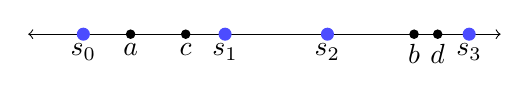
\begin{tikzpicture}
        \draw[<->] (-3,0) -- (3,0); 
        \filldraw[blue!70] (-2.3,0) circle (0.5ex) node[below] {$\textcolor{black}{s_0}$};
        \filldraw[blue!70] (-0.5,0) circle (0.5ex) node[below] {$\textcolor{black}{s_1}$};
        \filldraw[blue!70] (0.8,0) circle (0.5ex) node[below] {$\textcolor{black}{s_2}$};
        \filldraw[blue!70] (2.6,0) circle (0.5ex) node[below] {$\textcolor{black}{s_3}$};

        \filldraw[black] (-1.7,0) circle (0.35ex) node[below] {$\textcolor{black}{a}$};
        \filldraw[black] (-1,0) circle (0.35ex) node[below] {$\textcolor{black}{c}$};
        \filldraw[black] (1.9,0) circle (0.35ex) node[below] {$\textcolor{black}{b}$};
        \filldraw[black] (2.2,0) circle (0.35ex) node[below] {$\textcolor{black}{d}$};
    \end{tikzpicture} 
\end{center}

Clearly in this case we have that $I \cap S = J \cap S$. Now observe that 
\[
    \beta_a^b = \beta_c^d   
\]
since these intervals observe the same changes in rank.

\textcolor{NavyBlue}{Therefore, we see that the rank function 
for a tame function $f: \mathbb{R} \to X$ is $S$-constructible.}

\begin{definition}
    A map $Y: \textbf{Dgm} \to G$ is \textbf{$S$-finite} if 
    \[
        Y(I) \ne e \implies I = [s_i, s_j) \text{ or } I = [s_i, \infty)
    \]
    Alternatively, this states that 
    \[
        I \ne [s_i, s_j) \text{ and } I \ne [s_i, \infty) \implies Y(I) = e.
    \]
    which is probably a better way of thinking about this. 
\end{definition}

This leads to the following definition: 
\begin{definition}
    A \textbf{persistence diagram} is a finite map $Y: \textbf{Dgm} \to G$. 
\end{definition}

The motivation for this is due to the persistence diagram. Given a persistence diagram, 
we can extend it to a mapping 
\begin{align*}
    &X: \textbf{Dgm} \to \mathbb{Z}\\
    &[a, b) \mapsto \beta_{a_1}^{b_1} - \beta_{a_2}^{b_2} + \beta_{a_2}^{b_1} - \beta_{a_1}^{b_1}
\end{align*}
where $a_1 \le a \le a_2$ and $b_1 \le b \le b_2$ are values within some sufficiently 
small neighborhood of $a$ and $b$. Note that in this extension, if $[a, b) \ne [s_i, s_j)$ 
or $[s_i, \infty )$ in, then each $\beta_{a_i}^{b_j}$ is of full rank, so that 
\[
    X([a, b)) = 0.
\]
Hence we see that the persistence diagram is $S$-finite where $S$ is the finite set of
critical values. 

We now want to invent a distance between persistence diagrams. To do so, we must 
first denote $G$ as not only an abelian group, but one with a 
translational invariant partial ordering $\le$. What we mean by that is if 
$a \le b$ then $a + c \le b + c$ for any $a, b ,c \in G$. 

\begin{definition}
    Consider $Y_1, Y_2: \textbf{Dgm} \to G$ be a pair of persistence diagrams. 
    We say there exists a \textbf{morphism} $\phi: Y_1 \to Y_2$ if 
    \[
        \sum_{\substack{J \in \textbf{Dgm} \\ I \subset J}}Y_1(J) \le \sum_{\substack{J \in \textbf{Dgm} \\ I \subset J}}Y_2(J)
    \]
    for all $I \in \textbf{Dgm}$. 
\end{definition}

Note the above sums are finite.

\textcolor{NavyBlue}{Observe that if $\phi: Y_1 \to Y_2$ and $\phi': Y_2 \to Y_3$, 
then we can define the unique morphism $\phi' \circ \phi : Y_1 \to Y_3$. Therefore, 
this morphism relation establishes a reflexive, transitive ordering on our persistence diagrams.} 
Thus we can consider the category of persistence diagrams $\textbf{PDiag}(G)$ into the 
group $G$ where the objects are persistence diagrams $Y: \textbf{Dgm} \to G$ and morphisms 
as described above. As we stated before, these morphisms make this category 
into a partial ordering.

Define the mapping 
\begin{align*}
    \textbf{Grow}_\epsilon: \textbf{Dgm} &\to \textbf{Dgm}\\
    [p, q) &\mapsto [p - \epsilon, q + \epsilon] \text{ and } [p, \infty) \mapsto [p - \epsilon, \infty).
\end{align*}
Now consider a pair of persistence modules $Y_1, Y_2: \textbf{Dgm} \to G$. 
Since they are persistence modules, we know by definition that they are 
$S_1$ and $S_2$-finite for some finite sets $S_1, S_2$. With that said, observe that 
$Y_1 \circ \textbf{Grow}_\epsilon, Y_2 \circ \textbf{Grow}_\epsilon: \textbf{Dgm} \to G$ 
are again persistence modules since they $S_1'$ and $S_2'$ finite, where\dots

Therefore, we have an endofunctor on our category 
of persistence modules.
\begin{align*}
    \nabla_\epsilon : \textbf{PDgm}(G) \to \textbf{PDgm}(G)\\
    Y_1: \textbf{Dgm} \to G \mapsto Y_1 \circ \textbf{Grow}_\epsilon: \textbf{Dgm} \to G.
\end{align*}
Note that for any persistence modules $Y: \textbf{Dgm} \to G$, we have that 
$\nabla_\epsilon(Y) \to Y$ since for any interval $Y$, 
\[
    \sum_{\substack{J \in \textbf{Dgm} \\ I \subset J}}Y(J) 
    =
    Y_1 \circ \textbf{Grow}_\epsilon
\]
